\documentclass{article}\usepackage[]{graphicx}\usepackage[]{color}
% maxwidth is the original width if it is less than linewidth
% otherwise use linewidth (to make sure the graphics do not exceed the margin)
\makeatletter
\def\maxwidth{ %
  \ifdim\Gin@nat@width>\linewidth
    \linewidth
  \else
    \Gin@nat@width
  \fi
}
\makeatother

\definecolor{fgcolor}{rgb}{0.345, 0.345, 0.345}
\newcommand{\hlnum}[1]{\textcolor[rgb]{0.686,0.059,0.569}{#1}}%
\newcommand{\hlstr}[1]{\textcolor[rgb]{0.192,0.494,0.8}{#1}}%
\newcommand{\hlcom}[1]{\textcolor[rgb]{0.678,0.584,0.686}{\textit{#1}}}%
\newcommand{\hlopt}[1]{\textcolor[rgb]{0,0,0}{#1}}%
\newcommand{\hlstd}[1]{\textcolor[rgb]{0.345,0.345,0.345}{#1}}%
\newcommand{\hlkwa}[1]{\textcolor[rgb]{0.161,0.373,0.58}{\textbf{#1}}}%
\newcommand{\hlkwb}[1]{\textcolor[rgb]{0.69,0.353,0.396}{#1}}%
\newcommand{\hlkwc}[1]{\textcolor[rgb]{0.333,0.667,0.333}{#1}}%
\newcommand{\hlkwd}[1]{\textcolor[rgb]{0.737,0.353,0.396}{\textbf{#1}}}%
\let\hlipl\hlkwb

\usepackage{framed}
\makeatletter
\newenvironment{kframe}{%
 \def\at@end@of@kframe{}%
 \ifinner\ifhmode%
  \def\at@end@of@kframe{\end{minipage}}%
  \begin{minipage}{\columnwidth}%
 \fi\fi%
 \def\FrameCommand##1{\hskip\@totalleftmargin \hskip-\fboxsep
 \colorbox{shadecolor}{##1}\hskip-\fboxsep
     % There is no \\@totalrightmargin, so:
     \hskip-\linewidth \hskip-\@totalleftmargin \hskip\columnwidth}%
 \MakeFramed {\advance\hsize-\width
   \@totalleftmargin\z@ \linewidth\hsize
   \@setminipage}}%
 {\par\unskip\endMakeFramed%
 \at@end@of@kframe}
\makeatother

\definecolor{shadecolor}{rgb}{.97, .97, .97}
\definecolor{messagecolor}{rgb}{0, 0, 0}
\definecolor{warningcolor}{rgb}{1, 0, 1}
\definecolor{errorcolor}{rgb}{1, 0, 0}
\newenvironment{knitrout}{}{} % an empty environment to be redefined in TeX

\usepackage{alltt}
\IfFileExists{upquote.sty}{\usepackage{upquote}}{}
\begin{document}

COVID-19 has been spreading rapidly around the world. Italy has now gone into lock down, California has declared a state of emergency, schools and universities around the globe have canceled in person classes and events, and businesses have reduced travel and pushed work from home policies. All of this is designed to slow the spread of the disease. These efforts are broadly referred to as social distancing.

The idea is to reduce person-to-person contact in order to make spreading the disease less likely. The effects of this are often illustrated in images such as those in the chart below, where the red plot is flattened to spread out the disease as much as possible. This helps to ensure that there are sufficient resources available for a sick population, which will help improve survival rates.

Flattening the curve to keep infection manageable (Source: Fast.ai).
How do we determine the value of such distancing strategies and model this spread?


We walk through a SEIR epidemiological model and simulate it with R. The first model is the basic SEIR without social distancing, then we add social distancing to show how the potential effectiveness of these strategies.

The SEIR model is a compartmental model for modeling how a disease spreads through a population. It’s an acronym for Susceptible, Exposed, Infected, Recovered. When a disease is introduced to a population, the people move from one of these classes (or compartments) to the next. When they reach the R state, they’re no longer able to be infected, depending on your interpretation, they either survived the disease and are now immune or succumbed to the illness and are out of the population.

This is an extension of the classic SIR model and simply adds one more equation to show those who are exposed. The full model is given below:

We have four ODE's in the time domain, with three parameters: $\alpha$, $\beta$, $\gamma$.

\begin{itemize}

\item $\alpha$ is the inverse of the incubation period ($1/t_{incubation}$)
\item $\beta$ is the average contact rate in the population
\item $\gamma$ is the inverse of the mean infectious period ($1/t_{infectious}$)

\end{itemize}


Equation (1) is the change in people susceptible to the disease and is moderated by the number of infected people and their contact with the infected. Equation (2) gives the people who have been exposed to the disease. It grows based on the contact rate and decreases based on the incubation period whereby people then become infected.


\section{Create a bouncing ball}
\begin{knitrout}
\definecolor{shadecolor}{rgb}{0.969, 0.969, 0.969}\color{fgcolor}\begin{kframe}
\begin{alltt}
\hlstd{coord_range} \hlkwb{=} \hlkwd{c}\hlstd{(}\hlnum{0}\hlstd{,} \hlnum{1000}\hlstd{,} \hlnum{0}\hlstd{,} \hlnum{800}\hlstd{)}
\hlstd{N} \hlkwb{=} \hlnum{6}
\hlstd{tstep} \hlkwb{=} \hlnum{20}
\hlstd{location} \hlkwb{=} \hlnum{5}
\hlstd{(data_arr} \hlkwb{=} \hlkwd{array}\hlstd{(}\hlkwc{dim}\hlstd{=}\hlkwd{c}\hlstd{(tstep,location, N)))}
\end{alltt}
\begin{verbatim}
## , , 1
## 
##       [,1] [,2] [,3] [,4] [,5]
##  [1,]   NA   NA   NA   NA   NA
##  [2,]   NA   NA   NA   NA   NA
##  [3,]   NA   NA   NA   NA   NA
##  [4,]   NA   NA   NA   NA   NA
##  [5,]   NA   NA   NA   NA   NA
##  [6,]   NA   NA   NA   NA   NA
##  [7,]   NA   NA   NA   NA   NA
##  [8,]   NA   NA   NA   NA   NA
##  [9,]   NA   NA   NA   NA   NA
## [10,]   NA   NA   NA   NA   NA
## [11,]   NA   NA   NA   NA   NA
## [12,]   NA   NA   NA   NA   NA
## [13,]   NA   NA   NA   NA   NA
## [14,]   NA   NA   NA   NA   NA
## [15,]   NA   NA   NA   NA   NA
## [16,]   NA   NA   NA   NA   NA
## [17,]   NA   NA   NA   NA   NA
## [18,]   NA   NA   NA   NA   NA
## [19,]   NA   NA   NA   NA   NA
## [20,]   NA   NA   NA   NA   NA
## 
## , , 2
## 
##       [,1] [,2] [,3] [,4] [,5]
##  [1,]   NA   NA   NA   NA   NA
##  [2,]   NA   NA   NA   NA   NA
##  [3,]   NA   NA   NA   NA   NA
##  [4,]   NA   NA   NA   NA   NA
##  [5,]   NA   NA   NA   NA   NA
##  [6,]   NA   NA   NA   NA   NA
##  [7,]   NA   NA   NA   NA   NA
##  [8,]   NA   NA   NA   NA   NA
##  [9,]   NA   NA   NA   NA   NA
## [10,]   NA   NA   NA   NA   NA
## [11,]   NA   NA   NA   NA   NA
## [12,]   NA   NA   NA   NA   NA
## [13,]   NA   NA   NA   NA   NA
## [14,]   NA   NA   NA   NA   NA
## [15,]   NA   NA   NA   NA   NA
## [16,]   NA   NA   NA   NA   NA
## [17,]   NA   NA   NA   NA   NA
## [18,]   NA   NA   NA   NA   NA
## [19,]   NA   NA   NA   NA   NA
## [20,]   NA   NA   NA   NA   NA
## 
## , , 3
## 
##       [,1] [,2] [,3] [,4] [,5]
##  [1,]   NA   NA   NA   NA   NA
##  [2,]   NA   NA   NA   NA   NA
##  [3,]   NA   NA   NA   NA   NA
##  [4,]   NA   NA   NA   NA   NA
##  [5,]   NA   NA   NA   NA   NA
##  [6,]   NA   NA   NA   NA   NA
##  [7,]   NA   NA   NA   NA   NA
##  [8,]   NA   NA   NA   NA   NA
##  [9,]   NA   NA   NA   NA   NA
## [10,]   NA   NA   NA   NA   NA
## [11,]   NA   NA   NA   NA   NA
## [12,]   NA   NA   NA   NA   NA
## [13,]   NA   NA   NA   NA   NA
## [14,]   NA   NA   NA   NA   NA
## [15,]   NA   NA   NA   NA   NA
## [16,]   NA   NA   NA   NA   NA
## [17,]   NA   NA   NA   NA   NA
## [18,]   NA   NA   NA   NA   NA
## [19,]   NA   NA   NA   NA   NA
## [20,]   NA   NA   NA   NA   NA
## 
## , , 4
## 
##       [,1] [,2] [,3] [,4] [,5]
##  [1,]   NA   NA   NA   NA   NA
##  [2,]   NA   NA   NA   NA   NA
##  [3,]   NA   NA   NA   NA   NA
##  [4,]   NA   NA   NA   NA   NA
##  [5,]   NA   NA   NA   NA   NA
##  [6,]   NA   NA   NA   NA   NA
##  [7,]   NA   NA   NA   NA   NA
##  [8,]   NA   NA   NA   NA   NA
##  [9,]   NA   NA   NA   NA   NA
## [10,]   NA   NA   NA   NA   NA
## [11,]   NA   NA   NA   NA   NA
## [12,]   NA   NA   NA   NA   NA
## [13,]   NA   NA   NA   NA   NA
## [14,]   NA   NA   NA   NA   NA
## [15,]   NA   NA   NA   NA   NA
## [16,]   NA   NA   NA   NA   NA
## [17,]   NA   NA   NA   NA   NA
## [18,]   NA   NA   NA   NA   NA
## [19,]   NA   NA   NA   NA   NA
## [20,]   NA   NA   NA   NA   NA
## 
## , , 5
## 
##       [,1] [,2] [,3] [,4] [,5]
##  [1,]   NA   NA   NA   NA   NA
##  [2,]   NA   NA   NA   NA   NA
##  [3,]   NA   NA   NA   NA   NA
##  [4,]   NA   NA   NA   NA   NA
##  [5,]   NA   NA   NA   NA   NA
##  [6,]   NA   NA   NA   NA   NA
##  [7,]   NA   NA   NA   NA   NA
##  [8,]   NA   NA   NA   NA   NA
##  [9,]   NA   NA   NA   NA   NA
## [10,]   NA   NA   NA   NA   NA
## [11,]   NA   NA   NA   NA   NA
## [12,]   NA   NA   NA   NA   NA
## [13,]   NA   NA   NA   NA   NA
## [14,]   NA   NA   NA   NA   NA
## [15,]   NA   NA   NA   NA   NA
## [16,]   NA   NA   NA   NA   NA
## [17,]   NA   NA   NA   NA   NA
## [18,]   NA   NA   NA   NA   NA
## [19,]   NA   NA   NA   NA   NA
## [20,]   NA   NA   NA   NA   NA
## 
## , , 6
## 
##       [,1] [,2] [,3] [,4] [,5]
##  [1,]   NA   NA   NA   NA   NA
##  [2,]   NA   NA   NA   NA   NA
##  [3,]   NA   NA   NA   NA   NA
##  [4,]   NA   NA   NA   NA   NA
##  [5,]   NA   NA   NA   NA   NA
##  [6,]   NA   NA   NA   NA   NA
##  [7,]   NA   NA   NA   NA   NA
##  [8,]   NA   NA   NA   NA   NA
##  [9,]   NA   NA   NA   NA   NA
## [10,]   NA   NA   NA   NA   NA
## [11,]   NA   NA   NA   NA   NA
## [12,]   NA   NA   NA   NA   NA
## [13,]   NA   NA   NA   NA   NA
## [14,]   NA   NA   NA   NA   NA
## [15,]   NA   NA   NA   NA   NA
## [16,]   NA   NA   NA   NA   NA
## [17,]   NA   NA   NA   NA   NA
## [18,]   NA   NA   NA   NA   NA
## [19,]   NA   NA   NA   NA   NA
## [20,]   NA   NA   NA   NA   NA
\end{verbatim}
\begin{alltt}
\hlkwd{dimnames}\hlstd{(x)[[}\hlnum{1}\hlstd{]]} \hlkwb{<-} \hlkwd{c}\hlstd{(}\hlstr{"a"}\hlstd{,} \hlstr{"b"}\hlstd{)}  \hlcom{# assign 2nd dim names}
\end{alltt}


{\ttfamily\noindent\bfseries\color{errorcolor}{\#\# Error in dimnames(x)[[1]] <- c("{}a"{}, "{}b"{}): object 'x' not found}}\begin{alltt}
\hlkwd{dimnames}\hlstd{(data_arr)[[}\hlnum{2}\hlstd{]]} \hlkwb{<-} \hlkwd{c}\hlstd{(}\hlstr{"x"}\hlstd{,} \hlstr{"y"}\hlstd{,} \hlstr{"theta"}\hlstd{,} \hlstr{"speed"}\hlstd{,} \hlstr{"status"}\hlstd{)}
\hlstd{s}
\end{alltt}


{\ttfamily\noindent\bfseries\color{errorcolor}{\#\# Error in eval(expr, envir, enclos): object 's' not found}}\begin{alltt}
\hlcom{# Initialize Start Locations and Characteristics}
\hlstd{subj_x} \hlkwb{=} \hlkwd{runif}\hlstd{(N, coord_range[}\hlnum{1}\hlstd{],  coord_range[}\hlnum{2}\hlstd{]); subj_x}
\end{alltt}
\begin{verbatim}
## [1]  40.04757 751.55330 177.16122 666.26890 849.82270 638.44829
\end{verbatim}
\begin{alltt}
\hlstd{subj_y} \hlkwb{=} \hlkwd{runif}\hlstd{(N, coord_range[}\hlnum{3}\hlstd{],  coord_range[}\hlnum{4}\hlstd{]); subj_y}
\end{alltt}
\begin{verbatim}
## [1] 559.16849  73.21843 318.31420 315.74030 559.14225 465.48702
\end{verbatim}
\begin{alltt}
\hlstd{theta} \hlkwb{=} \hlkwd{round}\hlstd{(}\hlkwd{runif}\hlstd{(N,} \hlnum{0}\hlstd{,} \hlnum{360}\hlstd{),}\hlnum{0}\hlstd{); theta}
\end{alltt}
\begin{verbatim}
## [1] 190   2 103   6 256 357
\end{verbatim}
\begin{alltt}
\hlstd{speed} \hlkwb{=} \hlkwd{rep}\hlstd{(}\hlnum{5}\hlstd{,N)}
\hlstd{SERI} \hlkwb{=} \hlkwd{rep}\hlstd{(}\hlnum{0}\hlstd{, N); SERI[}\hlkwd{sample}\hlstd{(N,} \hlnum{1}\hlstd{)]} \hlkwb{=} \hlnum{1}\hlstd{; SERI}
\end{alltt}
\begin{verbatim}
## [1] 0 0 0 0 1 0
\end{verbatim}
\begin{alltt}
\hlstd{data_arr[}\hlnum{1}\hlstd{,,}\hlnum{1}\hlstd{]}
\end{alltt}
\begin{verbatim}
##      x      y  theta  speed status 
##     NA     NA     NA     NA     NA
\end{verbatim}
\begin{alltt}
\hlcom{#create function to move the subject}
\hlstd{move_x} \hlkwb{=} \hlkwa{function}\hlstd{(}\hlkwc{tstep}\hlstd{,} \hlkwc{subj}\hlstd{)\{}
\hlstd{data_arr[tstep,} \hlnum{4}\hlstd{, subj]} \hlopt{*} \hlkwd{cos}\hlstd{(data_arr[tstep,}\hlnum{3}\hlstd{, subj]}\hlopt{*}\hlstd{pi}\hlopt{/}\hlnum{180}\hlstd{)\}}
\hlstd{move_y} \hlkwb{=} \hlkwa{function}\hlstd{(}\hlkwc{tstep}\hlstd{,} \hlkwc{subj}\hlstd{)\{}
\hlstd{data_arr[tstep,} \hlnum{4}\hlstd{, subj]} \hlopt{*} \hlkwd{sin}\hlstd{(data_arr[tstep,}\hlnum{3}\hlstd{, subj]}\hlopt{*}\hlstd{pi}\hlopt{/}\hlnum{180}\hlstd{)\}}

\hlcom{# check function }
\hlcom{# move_y(1, 1); move_x(1,1)}

\hlcom{# move function}
\hlstd{move} \hlkwb{=} \hlkwa{function}\hlstd{(}\hlkwc{j}\hlstd{,} \hlkwc{i}\hlstd{)\{}
  \hlkwd{c}\hlstd{(data_arr[j}\hlopt{-}\hlnum{1}\hlstd{,} \hlnum{1}\hlstd{, i]}\hlopt{+} \hlkwd{move_x}\hlstd{(j}\hlopt{-}\hlnum{1}\hlstd{,i),}
    \hlstd{data_arr[j}\hlopt{-}\hlnum{1}\hlstd{,} \hlnum{2}\hlstd{, i]}\hlopt{+} \hlkwd{move_y}\hlstd{(j}\hlopt{-}\hlnum{1}\hlstd{,i),}
    \hlstd{data_arr[j}\hlopt{-}\hlnum{1}\hlstd{,} \hlnum{3}\hlstd{, i],}
    \hlstd{data_arr[j}\hlopt{-}\hlnum{1}\hlstd{,} \hlnum{4}\hlstd{, i],}
    \hlstd{data_arr[j}\hlopt{-}\hlnum{1}\hlstd{,} \hlnum{5}\hlstd{, i])}
\hlstd{\}}
\hlcom{# check addressing}
\hlcom{# data_arr[1,, 2]}

\hlkwa{for}\hlstd{(i} \hlkwa{in} \hlnum{1}\hlopt{:}\hlstd{N)\{}
  \hlcom{# Initial Locations}
  \hlstd{data_arr[}\hlnum{1}\hlstd{,,i]} \hlkwb{=} \hlkwd{c}\hlstd{(subj_x[i], subj_y[i], theta[i], speed[i], SERI[i])}
  \hlkwa{for}\hlstd{(j} \hlkwa{in} \hlnum{2}\hlopt{:}\hlstd{tstep)\{}
    \hlcom{# move subjects based on theta and speed}
    \hlstd{data_arr[j,,i]} \hlkwb{=} \hlkwd{move}\hlstd{(j, i)}
    \hlcom{# coarse corrections when hitting a boundary}
    \hlcom{# Min x-boundary}
    \hlkwa{if}\hlstd{(data_arr[j,}\hlnum{1}\hlstd{,i]} \hlopt{<} \hlstd{coord_range[}\hlnum{1}\hlstd{])\{}
      \hlstd{data_arr[j}\hlopt{-}\hlnum{1}\hlstd{,}\hlnum{3}\hlstd{,i]}\hlkwb{=}\hlnum{180}\hlopt{-}\hlstd{data_arr[j}\hlopt{-}\hlnum{1}\hlstd{,}\hlnum{3}\hlstd{,i]}
      \hlstd{data_arr[j,,i]} \hlkwb{=} \hlkwd{move}\hlstd{(j,i)}
    \hlstd{\}}
    \hlcom{#Max x-boundary}
    \hlkwa{if}\hlstd{(data_arr[j,}\hlnum{1}\hlstd{,i]} \hlopt{>} \hlstd{coord_range[}\hlnum{2}\hlstd{])\{}
      \hlstd{data_arr[j}\hlopt{-}\hlnum{1}\hlstd{,}\hlnum{3}\hlstd{,i]}\hlkwb{=}\hlnum{180}\hlopt{-}\hlstd{data_arr[j}\hlopt{-}\hlnum{1}\hlstd{,}\hlnum{3}\hlstd{,i]}
      \hlstd{data_arr[j,,i]} \hlkwb{=} \hlkwd{move}\hlstd{(j,i)}
    \hlstd{\}}
    \hlcom{#Min y-boundary}
    \hlkwa{if}\hlstd{(data_arr[j,}\hlnum{2}\hlstd{,i]} \hlopt{<} \hlstd{coord_range[}\hlnum{3}\hlstd{])\{}
      \hlstd{data_arr[j}\hlopt{-}\hlnum{1}\hlstd{,}\hlnum{3}\hlstd{,i]}\hlkwb{=}\hlnum{360}\hlopt{-}\hlstd{data_arr[j}\hlopt{-}\hlnum{1}\hlstd{,}\hlnum{3}\hlstd{,i]}
      \hlstd{data_arr[j,,i]} \hlkwb{=} \hlkwd{move}\hlstd{(j,i)}
    \hlstd{\}}
    \hlcom{#Max y-boundary}
    \hlkwa{if}\hlstd{(data_arr[j,}\hlnum{2}\hlstd{,i]} \hlopt{>} \hlstd{coord_range[}\hlnum{4}\hlstd{])\{}
      \hlstd{data_arr[j}\hlopt{-}\hlnum{1}\hlstd{,}\hlnum{3}\hlstd{,i]}\hlkwb{=}\hlnum{360}\hlopt{-}\hlstd{data_arr[j}\hlopt{-}\hlnum{1}\hlstd{,}\hlnum{3}\hlstd{,i]}
      \hlstd{data_arr[j,,i]} \hlkwb{=} \hlkwd{move}\hlstd{(j,i)}
    \hlstd{\}}
   \hlcom{# print(data_arr)}
  \hlstd{\}}
  \hlcom{#print(data_arr)}
\hlstd{\}}
\end{alltt}
\end{kframe}
\end{knitrout}


\section{Plot Results}

\begin{knitrout}
\definecolor{shadecolor}{rgb}{0.969, 0.969, 0.969}\color{fgcolor}\begin{kframe}
\begin{verbatim}
## , , 1
## 
##                x        y theta speed status
##  [1,] 40.0475748 559.1685   190     5      0
##  [2,] 35.1235360 558.3002   190     5      0
##  [3,] 30.1994973 557.4320   190     5      0
##  [4,] 25.2754585 556.5638   190     5      0
##  [5,] 20.3514197 555.6955   190     5      0
##  [6,] 15.4273810 554.8273   190     5      0
##  [7,] 10.5033422 553.9590   190     5      0
##  [8,]  5.5793034 553.0908   190     5      0
##  [9,]  0.6552647 552.2226   -10     5      0
## [10,]  5.5793034 551.3543   -10     5      0
## [11,] 10.5033422 550.4861   -10     5      0
## [12,] 15.4273810 549.6178   -10     5      0
## [13,] 20.3514197 548.7496   -10     5      0
## [14,] 25.2754585 547.8814   -10     5      0
## [15,] 30.1994973 547.0131   -10     5      0
## [16,] 35.1235360 546.1449   -10     5      0
## [17,] 40.0475748 545.2766   -10     5      0
## [18,] 44.9716136 544.4084   -10     5      0
## [19,] 49.8956523 543.5402   -10     5      0
## [20,] 54.8196911 542.6719   -10     5      0
## 
## , , 2
## 
##              x        y theta speed status
##  [1,] 751.5533 73.21843     2     5      0
##  [2,] 756.5502 73.39292     2     5      0
##  [3,] 761.5472 73.56742     2     5      0
##  [4,] 766.5442 73.74192     2     5      0
##  [5,] 771.5411 73.91642     2     5      0
##  [6,] 776.5381 74.09091     2     5      0
##  [7,] 781.5350 74.26541     2     5      0
##  [8,] 786.5320 74.43991     2     5      0
##  [9,] 791.5289 74.61441     2     5      0
## [10,] 796.5259 74.78890     2     5      0
## [11,] 801.5228 74.96340     2     5      0
## [12,] 806.5198 75.13790     2     5      0
## [13,] 811.5167 75.31240     2     5      0
## [14,] 816.5137 75.48689     2     5      0
## [15,] 821.5107 75.66139     2     5      0
## [16,] 826.5076 75.83589     2     5      0
## [17,] 831.5046 76.01039     2     5      0
## [18,] 836.5015 76.18488     2     5      0
## [19,] 841.4985 76.35938     2     5      0
## [20,] 846.4954 76.53388     2     5      0
## 
## , , 3
## 
##              x        y theta speed status
##  [1,] 177.1612 318.3142   103     5      0
##  [2,] 176.0365 323.1860   103     5      0
##  [3,] 174.9117 328.0579   103     5      0
##  [4,] 173.7870 332.9297   103     5      0
##  [5,] 172.6622 337.8016   103     5      0
##  [6,] 171.5374 342.6734   103     5      0
##  [7,] 170.4127 347.5453   103     5      0
##  [8,] 169.2879 352.4171   103     5      0
##  [9,] 168.1632 357.2890   103     5      0
## [10,] 167.0384 362.1608   103     5      0
## [11,] 165.9137 367.0327   103     5      0
## [12,] 164.7889 371.9045   103     5      0
## [13,] 163.6642 376.7764   103     5      0
## [14,] 162.5394 381.6483   103     5      0
## [15,] 161.4147 386.5201   103     5      0
## [16,] 160.2899 391.3920   103     5      0
## [17,] 159.1651 396.2638   103     5      0
## [18,] 158.0404 401.1357   103     5      0
## [19,] 156.9156 406.0075   103     5      0
## [20,] 155.7909 410.8794   103     5      0
## 
## , , 4
## 
##              x        y theta speed status
##  [1,] 666.2689 315.7403     6     5      0
##  [2,] 671.2415 316.2629     6     5      0
##  [3,] 676.2141 316.7856     6     5      0
##  [4,] 681.1867 317.3082     6     5      0
##  [5,] 686.1593 317.8309     6     5      0
##  [6,] 691.1319 318.3535     6     5      0
##  [7,] 696.1046 318.8762     6     5      0
##  [8,] 701.0772 319.3988     6     5      0
##  [9,] 706.0498 319.9214     6     5      0
## [10,] 711.0224 320.4441     6     5      0
## [11,] 715.9950 320.9667     6     5      0
## [12,] 720.9676 321.4894     6     5      0
## [13,] 725.9402 322.0120     6     5      0
## [14,] 730.9128 322.5346     6     5      0
## [15,] 735.8854 323.0573     6     5      0
## [16,] 740.8580 323.5799     6     5      0
## [17,] 745.8307 324.1026     6     5      0
## [18,] 750.8033 324.6252     6     5      0
## [19,] 755.7759 325.1479     6     5      0
## [20,] 760.7485 325.6705     6     5      0
## 
## , , 5
## 
##              x        y theta speed status
##  [1,] 849.8227 559.1423   256     5      1
##  [2,] 848.6131 554.2908   256     5      1
##  [3,] 847.4035 549.4393   256     5      1
##  [4,] 846.1939 544.5878   256     5      1
##  [5,] 844.9843 539.7363   256     5      1
##  [6,] 843.7746 534.8849   256     5      1
##  [7,] 842.5650 530.0334   256     5      1
##  [8,] 841.3554 525.1819   256     5      1
##  [9,] 840.1458 520.3304   256     5      1
## [10,] 838.9362 515.4789   256     5      1
## [11,] 837.7266 510.6275   256     5      1
## [12,] 836.5170 505.7760   256     5      1
## [13,] 835.3074 500.9245   256     5      1
## [14,] 834.0978 496.0730   256     5      1
## [15,] 832.8882 491.2216   256     5      1
## [16,] 831.6786 486.3701   256     5      1
## [17,] 830.4689 481.5186   256     5      1
## [18,] 829.2593 476.6671   256     5      1
## [19,] 828.0497 471.8156   256     5      1
## [20,] 826.8401 466.9642   256     5      1
## 
## , , 6
## 
##              x        y theta speed status
##  [1,] 638.4483 465.4870   357     5      0
##  [2,] 643.4414 465.2253   357     5      0
##  [3,] 648.4346 464.9637   357     5      0
##  [4,] 653.4277 464.7020   357     5      0
##  [5,] 658.4209 464.4403   357     5      0
##  [6,] 663.4140 464.1786   357     5      0
##  [7,] 668.4072 463.9169   357     5      0
##  [8,] 673.4003 463.6553   357     5      0
##  [9,] 678.3935 463.3936   357     5      0
## [10,] 683.3866 463.1319   357     5      0
## [11,] 688.3798 462.8702   357     5      0
## [12,] 693.3729 462.6085   357     5      0
## [13,] 698.3661 462.3469   357     5      0
## [14,] 703.3592 462.0852   357     5      0
## [15,] 708.3524 461.8235   357     5      0
## [16,] 713.3455 461.5618   357     5      0
## [17,] 718.3387 461.3001   357     5      0
## [18,] 723.3318 461.0385   357     5      0
## [19,] 728.3249 460.7768   357     5      0
## [20,] 733.3181 460.5151   357     5      0
\end{verbatim}
\end{kframe}
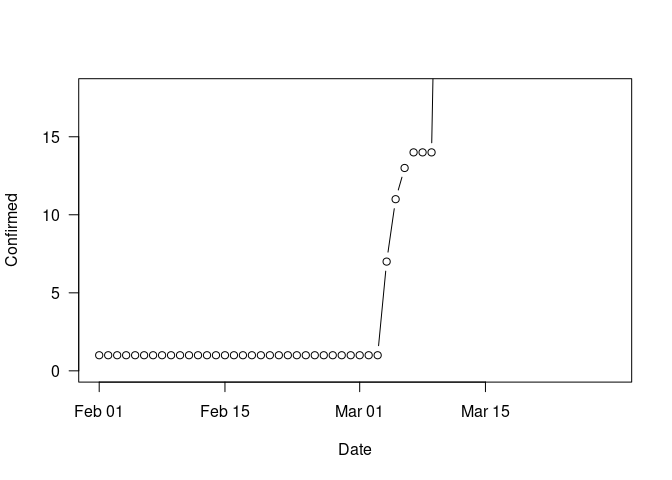
\includegraphics[width=\maxwidth]{figure/unnamed-chunk-2-1} 

\end{knitrout}

\end{document}
